\section{Non-increasing convex densities}\seclabel{convex}

Recall that $\sG_k$ is the class of non-increasing convex densities
supported on $\{1, \dots, k\}$. Then, $\sG_k$ forms a subclass of
$\sF_k$, which we considered in \secref{monotone}. This section is
devoted to extending the techniques of \secref{monotone} in order to
obtain a minimax rate upper bound on $\sG_k$. Again, the lower bound
is proved using standard techniques in \appref{convex-lower}.

In this section, we assume that $k$ is a power of three. In order to
prove the upper bound of \thmref{convex-result}, we construct a
ternary tree just as in \secref{monotone}, now with a ternary
splitting rule, where if a node $u$ has children $v, w, r$ in order
from left to right, we split and recurse if
\begin{equation}
  f_v - 2 f_w + f_r > \sqrt{\frac{f_v + f_w + f_r}{n}} . \eqlabel{convex-splitting-rule}
\end{equation}
Here we obtain a tree $T^\dagger = T^\dagger(f)$ with leaves
$L^\dagger$. If $u \in L^\dagger$ has children $v, w, r$ from left to
right, let $m_z$ be the midpoint of $I_z$ for $z \in \{v, w, r\}$. Let
the estimate $f^\dagger_n$ on $I_u$ be the line passing through the
points $(m_v, \bar{f}_v)$ and $(m_r, \bar{f}_r)$. Again, if
$|I_u| = 1$, then $f^\dagger_n(x) = f(x)$. We refer to $f_n^\dagger$
as the \emph{idealized tree-based estimate} for $f$.
\begin{rem}
  Since $f$ is non-increasing, the operation of \remref{birge-op} can
  again by applied to $f_n^\dagger$ to obtain a non-increasing
  estimate ${f_n^\dagger}'$ for which
  \[
    \TV({f_n^\dagger}', f) \le \TV(f_n^\dagger, f) .
  \]
\end{rem}

\begin{prop}\proplabel{conv-id-tv}
  \[
    \TV(f_n^\dagger, f) \le \frac{41}{48} \sqrt{\frac{|\{u \in L^\dagger \colon |I_u| > 1\}|}{n} } .
  \]
\end{prop}
Before proving this, we first note that by convexity of $f$, the slope
of the line passing through $(m_w, \bar{f}_w)$ and $(m_r, \bar{f}_r)$
is at least the slope of the line passing through $(m_v, \bar{f}_v)$
and $(m_w, \bar{f}_w)$. Equivalently,
\[
  f_r - f_w \ge f_w - f_v \iff f_v - 2 f_w + f_r \ge 0 .
\]
\begin{proof}[Proof of \propref{conv-id-tv}]
  \begin{figure} 
    \centering
    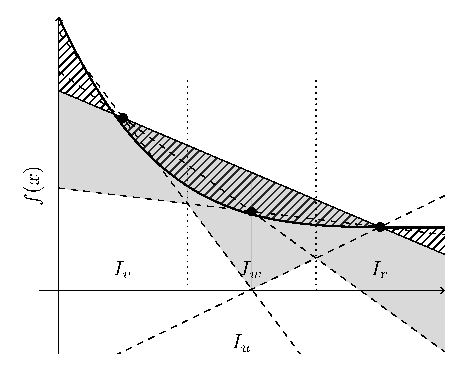
\includegraphics{convexplot.eps}
    \caption{A visualization of the $L_1$ distance between $f^\dagger_n$ and
      $f$ on $I_u$.}
    \figlabel{convexarea}
  \end{figure}  
  As in the proof of \propref{id-tv}, we have
  \[
    \TV(f_n^\dagger, f) = \frac{1}{2} \sum_{u \in L^\dagger \colon |I_u| > 1} A_u ,
  \]
  for $A_u = \sum_{x \in I_u} |f_n^\dagger(x) - f(x)|$. We refer to
  \figref{convexarea} for a visualization of the quantity $A_u$, which
  is depicted as the patterned area.

  %Let $B_v$, $B_w$, and $B_r$ denote the gray area on $I_v$, $I_w$,
  %and $I_r$ respectively. It can be shown that
  %\[
  %  A_u \le 2B_v + B_w + 2B_r ,
  %\]
  %and
  %\[
  %  B_v = B_r = (f_v - 2 f_w + f_r)/3 , \quad B_w = 3 (f_v - 2 f_w + f_r)/8 ,
  %\]
  %whence
  %\[
  %  A_u \le 2(f_v - 2 f_w + f_r) .
  %\]
  %The result then follows from the splitting rule
  %\eqref{convex-splitting-rule} and the Cauchy-Schwarz inequality.

  For $z \in \{v, w, r\}$, write
  \[
    B_z = \sum_{x \in I_z} |f^\dagger_n(x) - f(x)| .
  \]
  By convexity of $f$,
  \[
    B_w = \sum_{x \in I_w} (f^\dagger_n(x) - f(x)) .
  \]
  Observe also by convexity that $f(m_w) \ge \bar{f}_w$ and
  $f(m_r) \ge \bar{f}_r$. So, the line segment between
  $(m_w, \bar{f}_w)$ and $(m_r, \bar{f}_r)$ lies above $f$. Let
  $g_{wr} \colon \R \to \R$ be the line passing through the points
  $(m_w, \bar{f}_w)$ and $(m_r, \bar{f}_r)$. Then,
  \[
    \int_{I_w} g_{wr} = \bar{f}_w |I_w| = f_w ,
  \]
  Let $m_{wr}$ be the midpoint of $m_w$ and $m_r$, and $m_{vw}$ be the
  midpoint of $m_v$ and $m_w$. Let $x_w \in [-\infty, m_{wr}]$ be the
  leftmost point where $g_{wr}$ intersects $f$, if at all. Then,
  \[
    \int_{I_w \cap (-\infty, x_w]} (f - g_{wr}) = \int_{I_w \cap (x_w, \infty)} (g_{wr} - f),
  \]
  Since the right-hand side is non-negative, then indeed $x_w \in I_w$
  and it must be that $f$ lies above $g_{wr}$ to the left of
  $x_w$. Similarly, if $x_w' \in [m_{vw}, \infty]$ denotes the
  rightmost point where the line $g_{vw} \colon \R \to \R$ passing
  through $(m_v, \bar{f}_v)$ and $(m_w, \bar{f}_w)$ intersects $f$,
  then $x_w' \in I_w$ and $f$ lies above $g_{vw}$ to the right of
  $x_w'$. Therefore,
  \begin{align*}
    B_w &\le \int_{I_w \cap (-\infty, m_w]} (f^\dagger_n - g_{vw}) + \int_{I_w \cap (m_w, \infty)} (f^\dagger_n - g_{wr}) \\
        &= 3(f_v - 2 f_w + f_r)/8 .
  \end{align*}

  It remains to bound $B_v$ and $B_r$. Let $x_v \in I_v$ be the point
  where the line passing through $(m_v, \bar{f}_v)$ and
  $(m_r, \bar{f}_r)$ intersects $f$. As before, this points exists,
  and since $f$ is non-increasing, $x_v \le m_v$. Futhermore,
  \begin{align*}
    B_v &= \int_{I_v \cap (-\infty, x_v]} (f - f^\dagger_n) + \int_{I_v \cap (x_v, \infty)} (f^\dagger_n - f) \\
        &= 2 \int_{I_v \cap (x_v, \infty)} (f^\dagger_n - f) \\
        &\le 2 \int_{I_v} (f^\dagger_n - g_{wr}) \\
        &= 2(f_v - 2f_w + f_r)/3 ,
  \end{align*}
  where the inequality follows from convexity and earlier remarks. A
  similar argument follows for $B_r$.

  In total,
  \[
    A_u = B_v + B_w + B_r \le 41(f_v - 2 f_w + f_r)/24 .
  \]
  The result then follows from the splitting rule
  \eqref{convex-splitting-rule} and the Cauchy-Schwarz inequality.
\end{proof}

\begin{prop}
  If $n \ge 3^{10}$ and $3 n^{1/5} \le k < n^{1/5} 3^n$, then
  \[
    |L^\dagger| \le 34 n^{1/5} {\left( \log_3 (k/n^{1/5})\right)}^{4/5} .
  \]
\end{prop}
\begin{proof}
  The tree $T^\dagger$ has height at most $\log_3 k$. Let $U_j$ be the
  set of nodes at depth $j - 1$ in $T^\dagger$ with at least one leaf
  as a child, for $1 \le j \le \log_3 k$, labelled in order of
  appearance from right to left in $T^\dagger$ as
  $u_1, u_2, \dots, u_{3 |U_j|}$.
  %and let $V_j' \subseteq V_j$ be the set
  %of such nodes whose children are all leaves, or whose left and right
  %children are leaves. Let $V_j'' = V_j \setminus V_j'$. Order the
  %nodes in $V_j'$ in order of appearence from right to left in $T^*$
  %as $u_1, u_2, \dots, u_{|V_j'|}$.
  By the convex splitting rule \eqref{convex-splitting-rule}, and
  since $f$ is non-increasing,
  \[
    f_{u_3} - f_{u_2} > f_{u_2} - f_{u_1} + \sqrt{\frac{f_{u_1} + f_{u_2} +
        f_{u_3}}{n}} \ge \sqrt{\frac{f_{u_3} - f_{u_2}}{n}} ,
  \]
  so in particular, $f_{u_3} - f_{u_2} > 1/n$, and $f_{u_3} > 1/n$. In
  general,
  %\begin{align*}
  %  f_{u_{3i}} - f_{u_{3i - 1}} &> f_{u_{3(i - 1)}} - f_{u_{3(i - 1) - 1}} + \sqrt{f_{u_{3i
  %\end{align*}
  \begin{align}
    f_{u_{3i}} - f_{u_{3i - 1}} &> f_{u_{3(i - 1)}} - f_{u_{3(i - 1) - 1}} + \sqrt{ \frac{3 f_{u_{3(i - 1)}}}{n}} \notag \\
                                &\ge f_{u_{3(i - 1)}} - f_{u_{3(i - 1) - 1}} + \sqrt{\frac{3 \sum_{j = 1}^{i - 1} (f_{u_{3j}} - f_{u_{3j - 1}})}{n}} . \eqlabel{concave-induction}
  \end{align}
  We claim now that $f_{u_{3i}} - f_{u_{3i - 1}} > \frac{i^3}{27n}$,
  which we prove by induction; the base case is shown above, and by
  the induction hypothesis,
  \begin{align*}
    \eqref{concave-induction} &\ge \frac{(i - 1)^3}{27n} + \sqrt{\frac{3 \sum_{j = 1}^{i - 1} (j^3/27n)}{n}} \\
                              &\ge \frac{(i - 1)^3}{27n} + \frac{(i - 1)^2}{6n} \\
                              &\ge \frac{i^3}{27n} ,
  \end{align*}
  for all $i \ge 4$, while the cases $i = 2, 3$ can be manually
  verified. Then, by monotonicity of $f$,
  \begin{align}
    f_{u_{3i}} &> \frac{i^3}{27n} + f_{u_{3i - 1}} \notag \\
               &\ge \frac{i^3}{27n} + f_{u_{3(i - 1)}} \notag \\
               &\ge \sum_{j = 1}^i \frac{j^3}{27n} \notag \\
               &\ge \frac{i^4}{108 n} . \eqlabel{concave-prob-lower}
  \end{align}
  Let now $L_j$ be the set of leaves at level $j$ in $T^\dagger$. The
  leaves at level $j$ in order from right to left form a subsequence
  $v_1, \dots, v_{|L_{j}|}$ of $u_1, \dots, u_{3|U_j|}$. Let $q_j$ be
  the total probability mass of $f$ held in the leaves $L_j$. By
  \eqref{concave-prob-lower} and since $f_{v_i} \ge f_{u_i}$ for each
  $i$,
  \begin{align*}
    q_j \ge \sum_{i = 1}^{\floor{|L_j|/3}} f_{u_{3i}} \ge \sum_{i = 1}^{\floor{|L_j|/3}} \frac{i^4}{108n} \ge \frac{(\floor{|L_j|/3})^5}{540 n} ,
  \end{align*}
  so that
  \[
    |L_j| \le 3 + 3 (540 n q_j)^{1/5} \le 3 + 11 (n q_j)^{1/5} .
  \]
  Summing over all leaves,
  \begin{align*}
    |L^\dagger|  &\le n^{1/5} + \sum_{j = \floor{(1/5) \log_3 n}}^{\log_3 k} |L_j| \\
                 &\le n^{1/5} + 6 \log_3 (k/n^{1/5}) + 11 n^{1/5} \sum_{j = \floor{(1/5) \log_3 n}}^{\log_3 k} q_j^{1/5} .
  \end{align*}
  By H\"{o}lder's inequality,
  \begin{align*}
    \sum_{j = \floor{(1/5) \log_3 n}}^{\log_3 k} q_j^{1/5} &\le {\left( \sum_{j = 0}^{\log_3 k} q_j \right)}^{1/5} {\left( \sum_{j = \floor{(1/5) \log_3 k}}^{\log_3 k} 1 \right)}^{4/5} \\
                                                               &\le {\left(3 \log_3 (k/n^{1/5}) \right)}^{4/5} ,
  \end{align*}
  so finally
  \begin{align*}
    |L^\dagger| &\le n^{1/5} + 6 \log_3 (k/n^{1/5}) + 27 n^{1/5} {\left(\log_3 (k/n^{1/5})\right)}^{4/5} \\
                &\le 34 n^{1/5} {\left(\log_3 (k/n^{1/5}) \right)}^{4/5} . \qedhere
  \end{align*}
\end{proof}

\begin{proof}[Proof of the upper bound in \thmref{convex-result}]
  The proof is similar to that of \thmref{monotone-result}.
\end{proof}

\begin{rem}
  As in \remref{cont-monotone}, the argument can replicated in the
  continuous case, for bounded non-increasing convex densities
  supported on $[0, 1]$.
\end{rem}
